% !TEX TS-program = pdflatexmk
% !BIB TS-program = bibtex

\documentclass[12pt, a4paper, twoside]{book}
\usepackage{import}
\subimport{../}{preamble}
\ExecuteBibliographyOptions{articletitle=false}
\standalonetrue
\onehalfspacing
\begin{document}

\chapter{Supplementary Theory}

%\section{Mie Theory}

%Mie theory \cite{mie1908} is...

%\begin{figure}[h]
%\centering
%\includegraphics{figures/mie_scattering_ag}
%\caption[Mie scattering {\color{red}efficiencies/cross-sections} for AgNPs of increasing diameter]{\textbf{Mie scattering {\color{red}efficiencies/cross-sections} for AgNPs of increasing diameter.} The \SI{360}{nm} resonance position of the dipolar LSP mode of a AgNP in the quasistatic approximation is indicated by the dotted line. The resonance stays at \SI{360}{nm} until $d>\SI{60}{nm}$ then redshifts. The emergence of higher order modes following a similar behaviour is seen once $d>\SI{100}{nm}$.}
%\label{fig:mie_scattering_ag}
%\end{figure}

\section{Quantum Charge Transport}

One of main discussions of this work is the effect of quantum charge transport on plasmon coupling. Both quantum tunnelling and ballistic transport are qualitatively described in the main text for simplicity. The following section shows the relevant mathematical derivations of the simplest cases of quantum tunnelling and ballistic transport.

\subsection{Quantum Electron Tunnelling}

\subsection{Ballistic Conduction}

A 1D constriction between two charge reservoirs of length $L$ and width $W$ can be described as either diffusive if $l,l_\phi \ll L,W$, ballistic if $l,l_\phi \gg L,W$, or quasi-ballistic if inbetween, where $l$ and $l_\phi$ are the mean free path and phase coherence length, respectively. Conductance in the diffusive regime is as classically expected, $G=\sigma_{2D}W/L$. In the ballistic regime, however, it inherits quantum properties as is thus given by the Landauer formula,
\begin{equation} G=\frac{2e^2}{h}T(E_F), \end{equation}
where $T(E_F)$ is the transmission coefficient of an electron at the Fermi level. This is derived from the current flowing through a barrier between two biased reservoirs, whereby the Fermi levels are related via $E_{F,L} - E_{F,R} = eV$. The leftwards current through a barrier is given by,
\begin{equation}
	I_L = 2e \int_0^\infty f(E(k), E_{F,L}) v(k) T(k) \frac{dk}{2\pi},
	\label{eq:left_ballistic_current}
\end{equation}
where $f(E, E_F)$ is the Fermi-Dirac function and the wavevector of an electron can be related to its energy via $dE = \hbar v dk$. Converting \eqref{eq:left_ballistic_current} to an energy basis and adding the rightwards current yields,
\begin{equation}
	I_L = \frac{2e}{h} \int_{E_{L}}^\infty \left[ f(E(k), E_{F,L}) - f(E(k), E_{F,R}) \right] T(E) dE.
	\label{eq:ballistic_barrier_current}
\end{equation}
In the small bias limit%
\footnote{Large biases are ignored}
the Fermi-Dirac function is expanded as a Taylor series into,
\begin{equation}
	f(E(k), E_{F,L}) - f(E(k), E_{F,R}) \approx eV \frac{\delta f(E(k), E_F)}{\delta E_F}.
\end{equation}
Substituting this into \eqref{eq:ballistic_barrier_current} yields the integral,
\begin{equation}
	I_L = \frac{2e^2V}{h} \int_{E_{L}}^\infty \left[ -\frac{\delta f}{\delta E} \right] T(E) dE.
\end{equation}
At low temperatures $\delta f/\delta E \rightarrow \delta(E-E_F)$ and the integral evaluates to,
\begin{equation}
	I_L = \frac{2e^2V}{h}T(E_F),
\end{equation}
from which the conductance $G=I/V$ is derived to be,
\begin{equation}
		G = \frac{2e^2}{h}T(E_F).
\end{equation}
With the barrier still in place this corresponds to a tunnelling conductance with $T(E_F)<1$. The point at which the barrier disappears ($E_{barrier} = E_F$) gives rise to $T(E) = 1$ and opens up a single quantised conductance channel. Adding additional $n$ sub-bands into the constriction continues to increase the conductance by its quantum, $2e^2/h$, and thus the conductance of a 1D \emph{conductive} junction can be expressed as,
\begin{equation}
	G = \frac{2e^2}{h}n.
\end{equation}

\FloatBarrier
\chapter{Supplementary Experimental Details}

\section{Supplementary Optical Details}

Features, design justifications and optics theory not essential to the main text are detailed here. The following paragraphs clarify the advantages of the reimaging technique, the limitations in choice of objective lens, beamsplitters and optical bench layout. Lastly, further useful information and optics characterisation, such as the range of laser powers, are presented.

\subsection{Optical Design}

\begin{figure}
\centering
\subimport{../3_test_rig_design/figures/}{reimaging_concept.pdf_tex}
\caption*
%[Concept of reimaging for beam alignment]
{\textbf{Concept of reimaging for beam alignment.} Adjusting the angle of the beam in a focal plane does not change the position of the focus in the image (front focal) plane but changes the position in the Fourier (back focal) plane. Adjusting the angle of the beam in a Fourier plane translates the position of the beam in the image plane without changing its angular components.}
\label{fig:reimaging_concept}
\end{figure}

The concept of reimaging, and its effect on beam alignment, is shown in \figurename~\ref{fig:reimaging_concept}. The ray diagrams show that the beam position in the focus can be adjusted by changing the angle of a mirror placed in the Fourier plane (in the case of the microscope the mirror directly after the DF stop). The shape of the beam, dictated by its angular distribution in Fourier space, is controlled by tilting a mirror in a focal plane (the mirror in the focus of the reimaging arm). The two mirrors provide independent control over the two main beam properties.

\begin{figure}[bt]
\centering
\includegraphics{figures/objective_comparison}
\caption*
%[Spectral comparison between VIS and IR objectives]
{\textbf{Spectral comparison between VIS and IR objectives.} The VIS objective is an Olympus $100\times$ 0.9\,NA MPlan BD dark-field objective whereas the IR objective is an Olympus $100\times$ 0.8\,NA MPlan bright-field objective.}
\label{fig:objective_comparison}
\end{figure}

The choice of objective was determined by the overall range over which a reference spectrum from a Ag mirror is valid. Two long working distance objectives suitable for single nanostructure spectroscopy were characterised for use in the microscope: a VIS and a IR objective. The raw spectra measured using each of the objectives is shown in \figurename~\ref{fig:objective_comparison}. The sharp cut-on at \SI{480}{nm} is due to the supercontinuum laser. The VIS objective clearly outperforms the IR objective below \SI{625}{nm}, though both objective counts are large enough to maintain a good reference signal. Overall, references using the VIS objective only extend marginally more below \SI{500}{nm}. However, the sharp \SI{700}{nm} cut-off in the VIS objective means that it is not suitable for spectra in the NIR. The reference signal of the VIS objective is only valid up until \SI{900}{nm} whereas the IR objective extends to \SI{1100}{nm}. The gain in spectral range means that the IR objective is chosen despite its lack of dark-field illumination for imaging.

\begin{figure}[bt]
\centering
\includegraphics{figures/fresnel_coefficients}
\caption*
%[Reflectance as a function of angle of incidence for glass-air interface]
{\textbf{Reflectance as a function of angle of incidence for glass-air interface.} Reflective is calculated from the fresnel coefficients. The refractive index of glass is assumed to be $n=1.5$. The inset shows a zoomed segment in the low reflectance regime.}
\label{fig:fresnel}
\end{figure}

Consideration was given when designing the optical layout to account for intensity differences in each linear polarisation. Reflection and transmission of an incident EM wave at an interface between two refractive media is characterised by the Fresnel equations, with reflectance given by,
\begin{align}
R_s &= \left| \frac{n_1\cos{\theta_i} - n_2\cos{\theta_t}}{n_1\cos{\theta_i} + n_2\cos{\theta_t}} \right|^2, \\
R_p &= \left| \frac{n_1\cos{\theta_t} - n_2\cos{\theta_i}}{n_1\cos{\theta_t} + n_2\cos{\theta_i}} \right|^2,
\end{align}
where the wave impinges on the interface at an angle $\theta_i$ and refracts into a transmitted angle $\theta_t$ due to the refractive index change from $n_1$ to $n_2$. The angles are related using $n_2\sin{\theta_t} = n_1\sin{\theta_i}$. As shown in \figurename~\ref{fig:fresnel}, there is a large difference in reflectance between linear polarisations at higher angles of incidence. The microscope is designed such that the $s$-polarisation corresponds to light polarised along the tip axis, maximising its transmission to the spectrometers.

\subsection{Optical Characterisation}

\begin{figure}[bt]
\centering
\includegraphics{figures/fianium_power}
\caption*
%[Fianium power incident on the back aperture of the objective as a function of driving current.]
{\textbf{Fianium power incident on the back aperture of the objective as a function of driving current.} The beam diameter is restricted to the size of the back aperture to accurately measure the power throughput without measuring extra power not transmitted to the sample plane. Error bars represent the precision (standard error) of 1000 repeat measurements at each power, hence they are small, however the large distribution of points shows that the power meter is only accurate to \SI{1}{mW}.}
\label{fig:fianium_power}
\end{figure}

The measured broadband power incident on the back aperture of the objective (removing the contribution from over-filling of the back aperture using an iris) is shown in \figurename~\ref{fig:fianium_power}. The power is measured using a thermopile bolometer (Coherent Powermax) with simultaneous measurements of the spectral counts of the $s$-polarised signal component summed between 400--\SI{1200}{nm}. The supercontinuum laser is driven with a d.a.c. of 1100 in most experiments. Under these conditions, less than \SI{1}{mW} is used to illuminate samples, enough that reflection from a reference substrate just under saturates the spectrometer counts. Assuming a spot size on \orderof{\SI{1}{\micro\metre}} means a focal intensity of \SI{e8}{\milli\watt\per\centi\metre\squared}. Sub-mW powers are sufficient to maintain good signals without risking damage to nanoscale samples.

% Fast spectroscopy
%The signal passed to the fast spectroscopy path is used to measure spectra on \si{\micro\second} time scales. Light passing through this path is linearly polarised along a pre-determined axis and focussed onto a shutter constructed from a disassembled hard drive. The hard drive is trigged electronically using a TTL pulse from the oscilloscope to synchronise spectra with an electrical signal. Upon triggering the shutter light transmits through to a monochromater with CCD (Horiba Triax 320 with Princeton Instrument Pixis 256E CCD). The trigger pulse also begins a kinetics acquisition on the CCD in which the pixels are streaked from the active region to the read array before being read out. Light is dispersed and focussed onto the end most row of pixels so that the streaking process builds up a spectral image over time.

%\subsection{Time-Resolved Spectroscopy}

%Time-resolved spectroscopy is achieved using a charge-shuffling CCD. Only the furthermost row of pixels is illuminated with the charge shifted one row at a time every exposure period until the entire CCD has been moved into the readout arrays. The time interval recorded during time-resolved spectroscopy is given by,
%\begin{equation} t_{\mathrm{range}} = 256 (t_{\mathrm{exposure}} + t_{\mathrm{shift}}), \end{equation}
%where $t_{\mathrm{exposure}}$ is the exposure period of each row of pixels and $t_{\mathrm{shift}}$ is the time taken to shift all pixels by one row. The shift rate is set to \SI{9.2}{\micro\second}.
%Continuous cleans are enabled despite the clean cycle affecting the start time of the acquisition. By only cleaning the single illuminated row the cleaning time can be minimised to \SI{10}{\micro\second}.

\section{Supplementary Electronics}

\begin{figure}[bt]
\centering
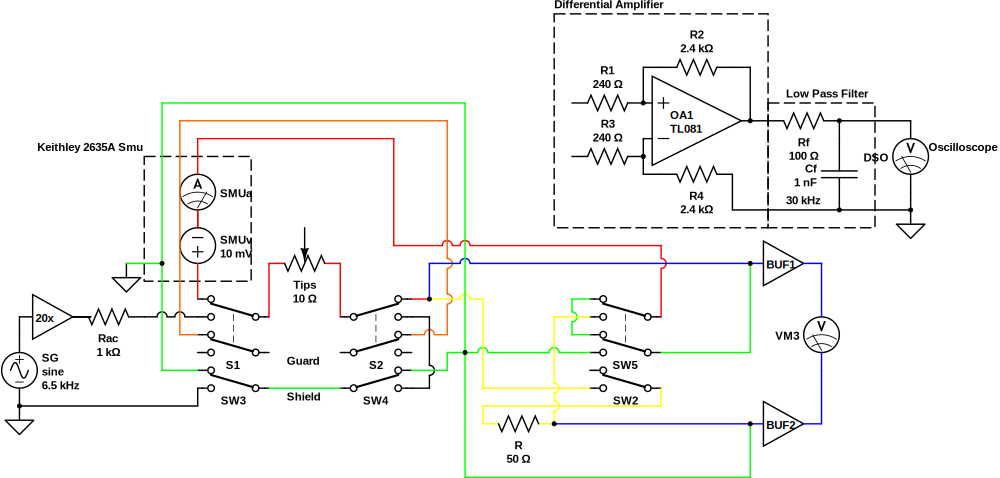
\includegraphics[width=0.9\textwidth]{figures/tip_experiment_circuit_design}
\caption[Schematic of the electrical measurement circuit.]{\textbf{Schematic of the electrical measurement circuit.} The central routing box allows switching between a.c.\ and d.c.\ circuits and low-and high-bandwidth d.c.\ measurements. The a.c.\ circuit is used to align two AFM probes together while the d.c.\ circuit is used to measure spatially dependent signals from the gap between two AFM probes.}
\label{fig:circuit_design}
\end{figure}

The circuitry of the microscope electronics is shown in \figref{fig:circuit_design}.

\section{Software Lock-In Derivation}

To lock into only the signal component at the reference frequency $\omega_r$ a reference wave needs to be computed. The first step in the lock-in process is to mathematically construct a single frequency waveform at the correct harmonic using the supplied reference signal. The reference signal is typically of the form $A\sin(\omega_{rs} t + \phi_r)$, but the algorithm will also work with any periodic function since it triggers off a rising position edge.
When $\sin(\theta)=0$ and the gradient is positive ($\cos(\theta)=1$) $\theta=2n\pi$. Hence the rising edge trigger points $t_i$ occur at,
\begin{equation} \theta = \omega_{rs} t_i + \phi_r = 2n\pi. \end{equation}
Trigger times are fitted against the number of triggers (number of periods) since the start of the signal using,
\begin{equation}
t_i = \frac{1}{\omega_{rs}}(2n\pi - \phi_r) = \frac{2\pi}{\omega_{rs}}n - \frac{\phi_r}{\omega_{rs}}.
\end{equation}
A complex reference wave of the form $e^{ih(\omega_{rs} t + \phi_r)}$, where $h$ is the harmonic of the reference frequency $\omega_{rs}$ required to lock into the frequency $\omega_r$, is constructed from the $t_i=mn+c$ fit using,
\begin{align}
\omega_{rs} &= \frac{2\pi}{m}, \\
\phi_r &= \frac{mc}{2\pi}.
\end{align}
The frequency component of the signal at $\omega_r=h\omega_{rs}$ can be extracted using Fourier analysis,
\begin{equation}
Z_s(\omega_r) = \frac{2}{t} \int_0^t{Z_s(t) e^{-ih(\omega_{rs} t + \phi_r)} dt}.
\end{equation}
Discretising this not a programmable form results in,
\begin{equation}
Z_s(\omega_r) = \frac{2}{n} \sum_0^n{Z_s(t_n) e^{-ih(\omega_{rs} t_n + \phi_r)}}
\end{equation}
where $\real{Z_s(\omega_r)}$ and $\imag{Z_s(\omega_r)}$ are the $x$ and $y$ of the signal component at $\omega_r$, respectively. Polar coordinates of amplitude and phase are retrieved using the coordinate transforms,
\begin{align}
r = \sqrt{x^2 + y^2}, \\
\phi = \tan^{-1}(y/x).
\end{align}

\section{Capacitive Alignment Model Derivation}

Beginning with the general equation of motion for two cantilevers, denoted by $i=(1,2)$, with initial positions $z_{0i}$, spring constants $k_{0i}^z$, masses $m_i$, damping coefficients $\beta_i^z$, and resonant frequencies $\omega_{0i} = \sqrt{k_{0i}/m_i}$, separated by a distance $d(t) = z_1(t) - z_2(t)$ and coupled via the $z$-components of the of the long range attractive electrostatic driving force $F_{EL}^z$ and short range (\orderof{nm}) Van da Waals and repulsive tip-tip interaction forces $F_{TT}^z$. The equilibrium separation between tips is denoted by $d_0 = z_{01} - z_{02}$. The equation of motion in the $z$-axis of the two parallel cantilevers of spring constant $k_i^z=k_{0i}^z+k_{TT}^z$ and damping coefficient $\beta_i^z=\beta_{0i}^z+\beta_{TT}^z$ is given by,
\begin{equation}
m_i\frac{d^2z_i}{dt^2}+\beta_i^z\frac{dz_i}{dt}+k_i^z\left(z_i-z_{0i}\right)=\pm\left(F_{EL}^z+F_{TT}^z\right),
\end{equation}
where the sign of the force depends on the tip - positive for one tip and negative for the other.
% Simplifications
Tip-tip interactions can be ignored and $F_{TT}^z = 0$ by assuming alignment takes place at long range and therefore $\beta_{TT}^{z} = k_{TT}^{z} = 0$. Further assume that one cantilever remains stationary. The apex separation is then restricted to $d=z_1$ with an equilibrium separation $d_0 = z_{01}$. Under these conditions the motion reduces to that of a single tip,
\begin{equation}
m_1\frac{d^2z_1}{dt^2}+\beta_1^z\frac{dz_1}{dt}+k_1^z\left(z_1-z_{01}\right) = F_{EL}^z(z_1, t).
\label{eq:simple_eom_app}
\end{equation}
The substitution $z_r = z_1-z_{01} = d-d_{0}$ can simplify the equation to using a single relative variable,
\begin{equation}
m_1 \frac{d^2z_r}{dt^2} + \beta_1^z \frac{dz_r}{dt} + k_1^zz_r = F_{EL}^z(z_r, t),
\end{equation}
This equation now describes the whole system rather than each individual tip with the main reference point between tips being the equilibrium separation $d_0$.

% Description of the electrostatic force
The remaining force exerted between tips is purely electrostatic and depends on voltage $V$ and capacitance $C$. In general an electrostatic force acting in one direction can be calculated using,
\begin{equation} F^z(V,z) = \frac{\partial U(V,z)}{\partial z}, \end{equation}
where the electrostatic potential is given by,
\begin{equation} U(V,z) = \frac{C(z)V^2}{2}. \end{equation}
The force is then given by,
\begin{equation} F_{EL}^z(V,z) = \frac{1}{2} \frac{\partial C(z)}{\partial z} V^2(t), \end{equation}
where $C(z)$ is the capacitance between the cantilevers when separated by a distance $d=z_1-z_2$ and $V(t)$ is the potential difference. Under the parallel plate capacitor model the capacitance is,
\begin{equation} C(z) = \frac{\varepsilon_0 A_{ov}}{z_1} + C_{bk}, \end{equation}
for plates with $A_{ov}$ area of overlap, including a stray capacitance $C_{bk}$. Applying a harmonic driving force at a frequency $\omega_s$,
\begin{equation} V(t)=V_0 \cos(\omega_s t), \end{equation}
results in a nonlinear driving force, given by,
\begin{equation} F_{EL}^z(z_1,t) = \frac{-\varepsilon_0 A_{ov} V(t)^2}{4z_1^2}. \end{equation}
The square of a harmonic signal doubles the frequency as per,
\begin{equation} V(t)^2 = V_0^2\cos^2(\omega_st) = \frac{V_0^2}{2}\left[1+\cos(2\omega_st)\right], \end{equation}
hence the driving force becomes,
\begin{equation}
	F_{EL}^z(z_1,t) = \left(\frac{-\varepsilon_0 A_{ov} V_0^2}{4z_1^2}\right)\left[1+\cos(\omega_pt)\right],
\label{eq:driving_force_app}
\end{equation}
where $\omega_p = 2\omega_s$ is the cantilever pump frequency.

% Deriving the final EoM of the simplified system
Substituting \eqref{eq:driving_force_app} into \eqref{eq:simple_eom_app} gives the simplified equation of motion for the dual-tip system,
\begin{equation}
	m_1 \frac{d^2z_1}{dt^2} + \beta_{01}^z \frac{dz_1}{dt} + k_{01}^z (z_1-d_0) = \left( \frac{-\varepsilon_0 A_{ov} V_0^2}{4z_1^2}\right)\left[1+\cos(\omega_pt)\right].
\label{eq:final_eom_app}
\end{equation}
Driving at a pump frequency close to the cantilever resonance ($\omega_p \approx \omega_{01}$) therefore leads to strong resonant oscillations between tips.
 
% Simplifying the final EoM using first order Taylor expansion of force
Expressing \eqref{eq:final_eom_app} in terms of $z_r$ and $d_0$ yields,
\begin{equation}
	m_1 \frac{d^2z_r}{dt^2} + \beta_{01}^z \frac{dz_r}{dt} + k_{01}^zz_r = \left( \frac{-\varepsilon_0 A_{ov} V_0^2}{4(z_r+d_0)^2}\right)\left[1+\cos(\omega_pt)\right],
\label{eq:final_rel_eom_app}
\end{equation}
and enables further simplification via approximation. Assuming that $z_r \ll d_0$ the right hand side of\eqref{eq:final_rel_eom_app} can be taken to first order using a Taylor series,%
\footnote{$F(z_r) = F(0) + \left.\frac{dF(z_r)}{dz_r}\right\rvert_0 z_r = \left(\frac{-\varepsilon_0 A_{ov} V_0^2}{4}\right) [1+\cos(\omega_pt)] \left(\frac{1}{d_0^2} - \frac{2z_r}{d_0^3 }\right)$}
%
\begin{equation}
m_1 \frac{d^2z_r}{dt^2} + \beta_{01}^z \frac{dz_r}{dt} + k_{e1}^zz_r \simeq \left(\frac{-\varepsilon_0 A_{ov} V_0^2}{4d_0^2}\right) \left[1+\cos(\omega_pt)\right],
\label{eq:first_order_eom_app}
\end{equation}
%
where,
%
\begin{equation}
k_{e1}^z = k_{01}^z - \left(\frac{\varepsilon_0 A_{ov} V_0^2}{2d_0^3}\right) \left[1+\cos(\omega_pt)\right].
\end{equation}
This effective spring constant $k_{e1}^z$ does not cause parametric mixing as it oscillates at $\omega_p$ and so its effect can be averaged out over time resulting in $\langle k_{e1}^{z} \rangle = k_{01}^z - {\varepsilon_0 A_{ov} V_0^2}/{2d_0^3}$. Defining the constant $q$ as,
\begin{equation} q = \left(\frac{-\varepsilon_0 A_{ov} V_0^2}{4d_0^3}\right), \end{equation}
the effective spring constant can be expressed as,
\begin{align}
k_{e1}^z &= k_{01}^z + 2q \left[1+\cos(\omega_pt)\right],\\
\langle k_{e1}^{z} \rangle &= k_{01}^z + 2q,
\end{align}
and the EOM can be again rewritten in the form,
\begin{equation}
m_1\ddot{z_r} + \beta_{01}^z\dot{z_r} + \left[\langle k_{e1}^z\rangle + 2q\cos(\omega_pt)\right]z_r - q\left[1+\cos(\omega_pt)\right]d_0 \simeq 0,
\label{eq:first_order_simple_eom_app}
\end{equation}
Equation \eqref{eq:first_order_simple_eom_app} is of the form of the driven damped Mathieu equation,
\begin{equation} \ddot{z} + 2\kappa\dot{z} + [a - 2q\cos(2t)]z = 0, \end{equation}
and has solutions in the limit of small oscillations of,
\begin{equation}
z_1 \approx d_0 - \left|z_{1}^{off}\right| - z_{m1}\cos(\omega_pt+\varphi_1)
\label{eq:tip_oscillation_app}
\end{equation}
where
\begin{subequations}
\begin{align}
z_1^{off} &\approx %
\frac{ \varepsilon_0 A_{ov} V_0^2 }{ 4d_0^2 \langle k_{e1}^z \rangle }, \label{eq:tip_amp_app}\\
%
z_{m1} &\approx %
\frac{ \varepsilon_0 A_{ov} V_0^2 }%
{ 4d_0^2 \sqrt{ (\langle k_{e1}^z \rangle - m_1\omega_p^2)^2 + (\beta_{01}^z\omega_p)^2  } }, \\
%
\varphi_1 &\approx \tan^{-1}\left(\frac{\beta_{01}^{z}\omega_{p}}{\langle k_{e1}^{z} \rangle -m_{1}\omega_{p}^{2}}\right). \label{eq:tip_phase_app}
\end{align}
\end{subequations}

When extending this to determine current flow, the general current through the tip junction is given by,
\begin{equation}
I(t) = \frac{dQ}{dt} = \frac{d(CV)}{dt} = C(t)\frac{dV(t)}{dt} + V(t)\frac{dC(t)}{dt}.
\end{equation}
Substituting for $C(t)$ and $V(t)$ and taking the first few terms in the Taylor series results in the first-order current flow,
\begin{subequations}
\begin{align}
I(\omega_{s}) & \approx \omega_{s}C_{0}V_{0} \left(1+\frac{|z_{off}|}{d_{0}}+\frac{z_{m1}}{2d_{0}}e^{i\varphi_1}+\frac{C_{bk}}{C_{0}}\right)e^{i\frac{\pi}{2}},\\
%
I(\omega_{p}+\omega_{s}) & \approx \frac{\left(\omega_{p}+\omega_{s}\right)C_{0}V_{0}z_{m1}}{2d_{0}} e^{i\left(\varphi_1 + \frac{\pi}{2}\right)},
\label{eq:3rd_harmonic_current_app}
\end{align}
\end{subequations}
where $C_0 = \varepsilon_0 A^{ov} / d_0$ and $z_{off}$ is an additional offset due to $F_{EL}^z \propto V^2$.

\subimport{./}{fast_spectroscopy}

\begin{singlespace}
\printbibliography[category=appendices, resetnumbers=true, title={Supplementary References}]
\end{singlespace}

\end{document}